\section{Prediction and cluster test results}\label{sec:testing}
To validated that the cluster gives us an improvement when working on big data, a list of tests will be explored. The first initial tests that will be performed, seen in \Cref{sec:initialtest}, will be run to find the settings the cluster should run with. In \Cref{sec:clustertest}, the tests run on the cluster and the results will be presented.

\subsection{Initial testing}\label{sec:initialtest}
In this section several tests will be performed which does not require the cluster. These tests will be run to find the settings the cluster should be run with when the final cluster tests will be performed.

\subsubsection{Best machine learning technique}
First the best machine learning technique needs to be identified. In this test six different methods are included, these are: naive bayes, hidden naive bayes, logistic regression, neural network, support vector machines(SVM) and adaboost. All the different methods are tested with multiple parameter settings to find the configuration that yields the best result. The feature representation used for this test is binary representation, presented in \Cref{sec:representationoffeatures}, and 35000 matches are used. The data will be split, using $\frac{2}{3}$ for training and $\frac{1}{3}$ for testing. 

The best accuracy of all the machine learning technique can be seen in \Cref{fig:besttech}. As seen, SVM and Neural networks has the worst accuracy, even after testing different parameter configurations. Naive bayes, adaboost and Hidden naive bayes all have comparable results around 56.5\%, but logistic regression has the best accuracy almost hitting 57\%, which will be the technique mainly used throughout these tests.  

% \begin{figure}[!htb]
%   \begin{tikzpicture}
%     \begin{axis}[
%       x tick label style={/pgf/number format/1000 sep=},
%       ylabel=Accuracy,
%       xlabel=Parameter configuration,
%       enlargelimits=0.05,
%       legend style={at={(0.5,1.1)},
%         anchor=north,legend columns=-1},
%       ybar interval=0.7,
%       width=.75\textwidth,
%       ymin=56, ymax=57,
%       ]
%       \addplot[fill=red] coordinates {(13,56.5462) 
%         (12,56.6218) 
%         (11,56.8403) 
%         (10,56.8319) 
%         (9,56.916) 
%         (8,56.8487) 
%         (7,56.8655) 
%         (6,56.6471) 
%         (5,56.6471) 
%         (4,56.605) 
%         (3,56.605) 
%         (2,56.5882) 
%         (1,56.5798) 
%         (0,2)
%       };
%       \addplot[fill=blue] coordinates {(13,56.4454) 
%         (12,56.4454) 
%         (11,56.4454) 
%         (10,56.4454) 
%         (9,56.4454) 
%         (8,56.4454) 
%         (7,56.4454) 
%         (6,56.4454) 
%         (5,56.4454) 
%         (4,56.4454) 
%         (3,56.4454) 
%         (2,56.4454) 
%         (1,56.4454) 
%         (0,56.4454)
%       };
%       \addplot[fill=green] coordinates {(13,56.6807) 
%         (12,56.6807) 
%         (11,56.6807) 
%         (10,56.6807) 
%         (9,56.6807) 
%         (8,56.6807) 
%         (7,56.6807) 
%         (6,56.6807) 
%         (5,56.6807) 
%         (4,56.6807) 
%         (3,56.6807) 
%         (2,56.6807) 
%         (1,56.6807) 
%         (0,56.6807)
%       };
%       \addplot[fill=orange] coordinates {(13,0) 
%         (12,0) 
%         (11,0) 
%         (10,0) 
%         (9,0) 
%         (8,49.87) 
%         (7,56.2269) 
%         (6,56.479) 
%         (5,56.1261) 
%         (4,55.5126) 
%         (3,54.7899) 
%         (2,54.5378) 
%         (1,53.7983) 
%         (0,2)
%       };
%       \addplot[fill=black] coordinates {(13,0) 
%         (12,0) 
%         (11,0) 
%         (10,0) 
%         (9,0) 
%         (8,0) 
%         (7,0) 
%         (6,0) 
%         (5,50.1) 
%         (4,55.6555) 
%         (3,52.7311) 
%         (2,55.5126) 
%         (1,50.2101) 
%         (0,0)
%       };
%       \addplot[fill=purple] coordinates {(13,0)
%         (12,0)
%         (11,0)
%         (10,0)
%         (9,0)
%         (8,0)
%         (7,0)
%         (6,0)
%         (5,0)
%         (4,55.3193)
%         (3,55.63)
%         (2,51.521)
%         (1,55.5714)
%         (0,0)
%       };
%       \legend{Logistic Regression,Naive Bayes,Hidden Naive Bayes,Adaboost,Neural Network,SVM}
%     \end{axis}
%   \end{tikzpicture}
%   \caption{Test of best machine learning technique}\label{fig:besttech}
% \end{figure}

\begin{figure}[!htb]
  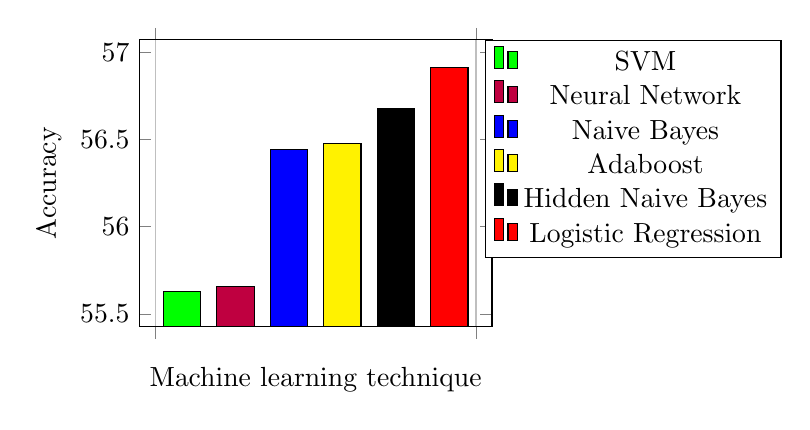
\begin{tikzpicture}
    \begin{axis}[
      %x tick label style={/pgf/number format/1000 sep=},
      xticklabel=\empty,
      ylabel=Accuracy,
      xlabel=Machine learning technique,
      enlargelimits=0.05,
      legend style={at={(1.4,1.0)},
        anchor=north,legend columns=1},
      ybar interval=0.7,
      width=.50\textwidth,
      ymin=55.5, ymax=57,
      reverse legend,
      ]
      \addplot[fill=red] coordinates {(1,56.916) 
        (0,2)
      };
      \addplot[fill=black] coordinates {(1,56.6807) 
        (0,56.6807)
      };
      \addplot[fill=yellow] coordinates {(1,56.479) 
        (0,2)
      };
      \addplot[fill=blue] coordinates {(1,56.4454) 
        (0,56.4454)
      };
      \addplot[fill=purple] coordinates {(1,55.6555) 
        (0,0)
      };
      \addplot[fill=green] coordinates {(1,55.63)
        (0,0)
      };
      \legend{Logistic Regression,Hidden Naive Bayes,Adaboost,Naive Bayes,Neural Network,SVM}
    \end{axis} 
  \end{tikzpicture}
  \caption{Test of best machine learning technique}\label{fig:besttech}
\end{figure}



\subsubsection{Implementation comparison}
To test if Apache Sparks PySpark implementation of logistic regression is implemented properly, it is compared to the equivalent implementations in Weka and R. The data consists of 5000 matches where Weka uses a sparse presentation, while R uses a dense and PySpark the raw file with JSON elements. As seen in \Cref{tab:impl_results}, the implementations are close to equal, the minor differences could be caused by differences in the parameter settings. However these results confirm that all implementations are acceptable and further testing can be performed in any of the environments.

\begin{table}[!htb]
  \centering
  \begin{tabular}{|l|c|}
    \hline
    Implementation  & Accuracy  \\
    \hline
    Weka & 55\%  \\
    R & 55\%\\
    PySpark & 53\%\\ 
    \hline
  \end{tabular}
  \caption{Implementation comparison results}
  \label{tab:impl_results}
\end{table}

\subsubsection{Feature representation test}
Features can be presented in many different ways and this test is constructed to finding the best way to that. The representations that will be tested are the methods presented in \Cref{sec:representationoffeatures}. The test was done on an increasing number of matches with all the different methods to check how they hold up with much data. As the result, shown in \Cref{fig:feat-rep}, indicates, method 1 and 4 are very close, but binary being slightly above ternary majority of the time, which is the reason for us choosing binary.

\begin{figure}[!htb]
  \centering
  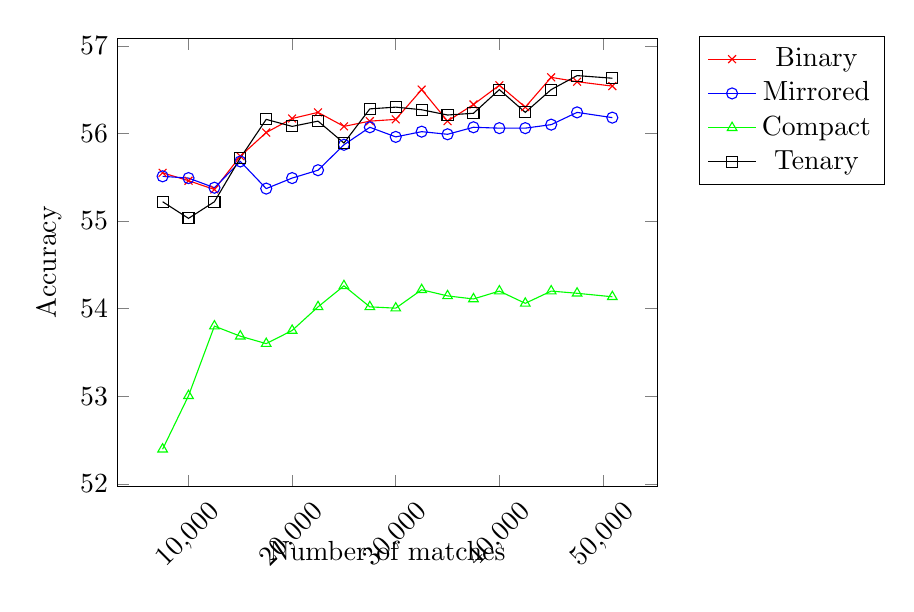
\begin{tikzpicture}[] 
    \begin{axis}[
      xlabel=Number of matches, 
      ylabel=Accuracy,
      xtick={10000,20000,30000,40000,50000},
      xticklabel style={rotate=45,anchor=near xticklabel},
      scaled x ticks=false,
      x label style={at={(axis description cs:0.5,-0.1)},anchor=north},
      legend style={at={(1.25,1.005)},
        anchor=north,legend columns=1},] 
      \addplot[color=red,mark=x] coordinates { 
        (7500, 55.55)
        (10000, 55.46)
        (12500, 55.36)
        (15000, 55.74)
        (17500, 56.01)
        (20000, 56.17)
        (22500, 56.24)
        (25000, 56.08)
        (27500, 56.14)
        (30000, 56.16)
        (32500, 56.50)
        (35000, 56.14)
        (37500, 56.33)
        (40000, 56.55)
        (42500, 56.30)
        (45000, 56.64)
        (47500, 56.59)
        (50901, 56.54)
      };
      \addplot[color=blue,mark=o] coordinates { 
        (7500, 55.51)  
        (10000, 55.49)
        (12500, 55.38)
        (15000, 55.68)
        (17500, 55.37)
        (20000, 55.49)
        (22500, 55.58)
        (25000, 55.87)
        (27500, 56.07)
        (30000, 55.96)
        (32500, 56.02)
        (35000, 55.99)
        (37500, 56.07)
        (40000, 56.06)
        (42500, 56.06)
        (45000, 56.10)
        (47500, 56.24)
        (50901, 56.18)
      };
      \addplot[color=green,mark=triangle] coordinates { 
        (7500, 52.395)  
        (10000, 53.005)
        (12500, 53.80)
        (15000, 53.685)
        (17500, 53.60)
        (20000, 53.75)
        (22500, 54.02)
        (25000, 54.26)
        (27500, 54.02)
        (30000, 54.005)
        (32500, 54.215)
        (35000, 54.145)
        (37500, 54.11)
        (40000, 54.20)
        (42500, 54.06)
        (45000, 54.20)
        (47500, 54.175)
        (50901, 54.135)
      };
      \addplot[color=black,mark=square] coordinates {
        (7500, 55.22)  
        (10000, 55.03)
        (12500, 55.22)
        (15000, 55.72)
        (17500, 56.16)
        (20000, 56.08)
        (22500, 56.14)
        (25000, 55.89)
        (27500, 56.28)
        (30000, 56.30)
        (32500, 56.27)
        (35000, 56.21)
        (37500, 56.23)        
        (40000, 56.50)
        (42500, 56.24)
        (45000, 56.50)
        (47500, 56.66)
        (50901, 56.63)
      };
      \legend{Binary, Mirrored, Compact, Tenary}
    \end{axis} 
  \end{tikzpicture}
  \caption{Test for representation of features}\label{fig:feat-rep}
\end{figure}

\subsubsection{Feature tests}\label{sec:feattest}
Some features might be more expressive than others, and finding the set of features that will yield the best result is imperative. Some more text about \Cref{fig:best-feat}.

\begin{figure}[!htb]
  \centering
  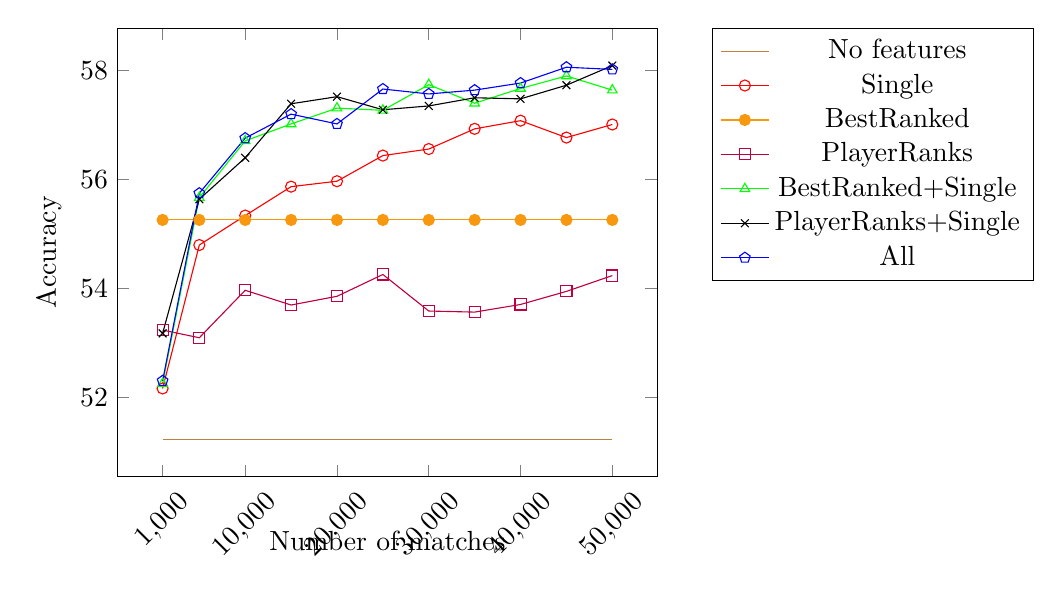
\begin{tikzpicture}[] 
    \begin{axis}[
      xlabel=Number of matches, 
      ylabel=Accuracy,
      xtick={1000,10000,20000,30000,40000,50000},
      xticklabel style={rotate=45,anchor=near xticklabel},
      scaled x ticks=false,
      x label style={at={(axis description cs:0.5,-0.1)},anchor=north},
      legend style={at={(1.4,1.001)},
        anchor=north,legend columns=1},] 
      \addplot[color=brown] coordinates { 
        (1000,51.24)
        (5000,51.24)
        (10000,51.24)
        (15000,51.24)
        (20000,51.24)
        (25000,51.24)
        (30000,51.24)
        (35000,51.24)
        (40000,51.24)
        (45000,51.24)
        (50000,51.24)
      };
      \addplot[color=red,mark=o] coordinates { 
        (1000,52.17)
        (5000,54.8)
        (10000,55.34)
        (15000,55.87)
        (20000,55.97)
        (25000,56.44)
        (30000,56.56)
        (35000,56.93)
        (40000,57.08)
        (45000,56.77)
        (50000,57.01)
      };
      \addplot[color=YellowOrange,mark=*] coordinates { 
        (1000,55.26)
        (5000,55.26)
        (10000,55.26)
        (15000,55.26)
        (20000,55.26)
        (25000,55.26)
        (30000,55.26)
        (35000,55.26)
        (40000,55.26)
        (45000,55.26)
        (50000,55.26)
      };
      \addplot[color=purple,mark=square] coordinates { 
        (1000,53.24)
        (5000,53.1)
        (10000,53.97)
        (15000,53.7)
        (20000,53.86)
        (25000,54.26)
        (30000,53.59)
        (35000,53.57)
        (40000,53.71)
        (45000,53.95)
        (50000,54.24)
      };
      \addplot[color=green,mark=triangle] coordinates { 
        (1000,52.26)
        (5000,55.67)
        (10000,56.71)
        (15000,57.02)
        (20000,57.31)
        (25000,57.27)
        (30000,57.74)
        (35000,57.4)
        (40000,57.67)
        (45000,57.9)
        (50000,57.64)
      };
      \addplot[color=black,mark=x] coordinates { 
        (1000,53.18)
        (5000,55.64)
        (10000,56.4)
        (15000,57.39)
        (20000,57.52)
        (25000,57.28)
        (30000,57.35)
        (35000,57.5)
        (40000,57.48)
        (45000,57.73)
        (50000,58.09)
      };
      \addplot[color=blue,mark=pentagon] coordinates { 
        (1000,52.31)
        (5000,55.75)
        (10000,56.76)
        (15000,57.2)
        (20000,57.02)
        (25000,57.66)
        (30000,57.57)
        (35000,57.64)
        (40000,57.77)
        (45000,58.06)
        (50000,58.02)
      };
      \legend{No features,Single,BestRanked,PlayerRanks,BestRanked+Single,PlayerRanks+Single,All}
    \end{axis} 
  \end{tikzpicture}
  \caption{Accuracy of features}\label{fig:best-feat}
\end{figure}

\subsection{Cluster tests}\label{sec:clustertest}
In this section the tests that requires the cluster. This is due to the size of the tests, and the expected time frame.
\subsubsection{Big data improvements}
To test if big data gives an improvement when predicting the outcome of a match, the same features and method where used on an increasing sized data starting from 1000 matches. After the model was made, it was tested on the training data, as a $\frac{2}{3}$-split and finally cross-validation. And as seen on \Cref{fig:bigdata} there will be more information once more tests has been run!

\begin{figure}[!htb]
  \centering
  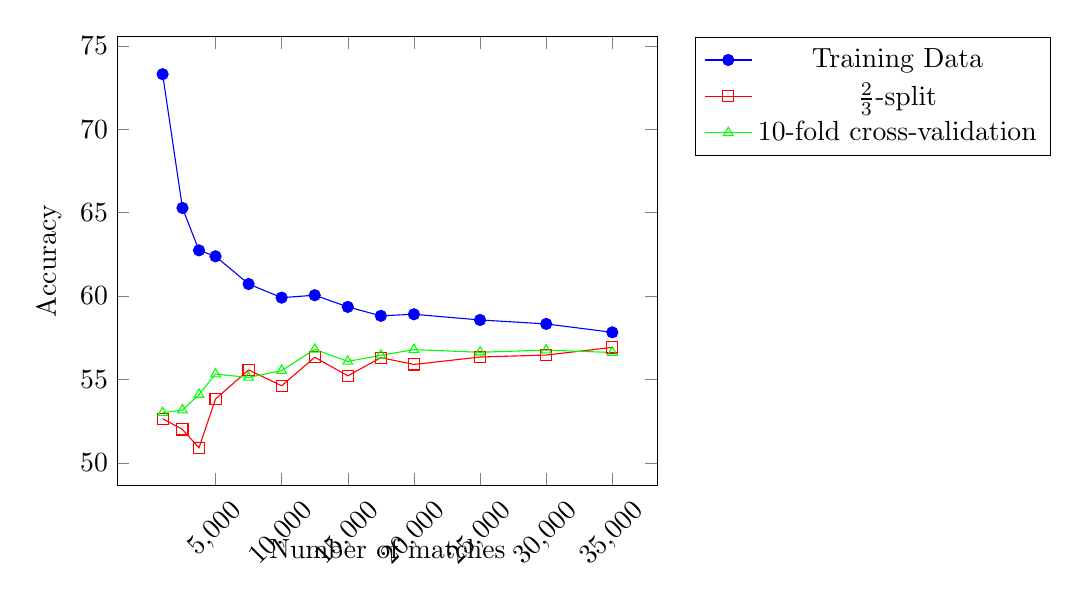
\begin{tikzpicture}[] 
    \begin{axis}[
      xlabel=Number of matches, 
      ylabel=Accuracy,
      xtick={5000,10000,15000,20000,25000,30000,35000},
      xticklabel style={rotate=45,anchor=near xticklabel},
      scaled x ticks=false,
      x label style={at={(axis description cs:0.5,-0.1)},anchor=north},
      legend style={at={(1.4,1.0)},
        anchor=north,legend columns=1},] 
      \addplot[color=blue,mark=*] coordinates {
        (1000, 73.3)   	
        (2500,65.28)  	
        (3750,62.7367)	
        (5000,62.38)
        (7500,60.72)
        (10000,59.9)
        (12500,60.048)
        (15000,59.3467)
        (17500,58.8114)
        (20000,58.905)
        (25000,58.564)
        (30000,58.3267)
        (35000,57.8229)
      };
      \addplot[color=red,mark=square] coordinates {
        (1000,52.6471)
        (2500,52)
        (3750,50.902)
        (5000,53.8235)
        (7500,55.5686)
        (10000,54.6176)
        (12500,56.3294)
        (15000,55.2157)
        (17500,56.3025)
        (20000,55.8971)
        (25000,56.3412)
        (30000,56.4608)
        (35000,56.916)
      };
      \addplot[color=green,mark=triangle] coordinates {
        (1000,53)
        (2500,53.16)
        (3750,54.0944)
        (5000,55.32)
        (7500,55.12)
        (10000,55.53)
        (12500,56.8)
        (15000,56.08)
        (17500,56.4457)
        (20000,56.785)
        (25000,56.628)
        (30000,56.7567)
        (35000,56.6143)
      };
      \legend{Training Data, $\frac{2}{3}$-split, 10-fold cross-validation}
    \end{axis} 
  \end{tikzpicture}
  \caption{Test for representation of features}\label{fig:bigdata}
\end{figure}

\subsubsection{Speed up}
This test is constructed to show that an increasing number of nodes increases the computation speed. As seen in \Cref{sec:clustersetup}, the cluster consists of 4 nodes, this means the test will be run with the master and either 1, 2 or 3 nodes. The data for this test be the same to make the results comparable.

\begin{table}[!htb]
  \centering
  \begin{tabular}{|c|c|}
    \hline
    Number of nodes & Time taken\\
    \hline
    1 & ? \\
    2 & ? \\
    3 & ? \\
    \hline
  \end{tabular}
  \caption{Speed up test results}\label{tab:speedup}
\end{table}

\subsubsection{Prediction with team ranks}
Previous seasons rank for each player is registered in the match data. This test is constructed to test whether this rank alone is a useful feature when predicting a winning team.
\subsubsection{Prediction with all features}
All the features created from the data is used for this test. 
\subsubsection{Prediction with all features except lane}
This test is almost identical to the test seen above, except the lane feature is excluded. This test is performed to learn if the lane each hero choses to defend influences the outcome of the match and if this is actually useful when predicting outcome of future matches.
\subsubsection{Prediction using support vector machine}
The above tests will for this test be performed using support vector machine to see how it compares to logistic regression. 
\subsubsection{Prediction with best features}
The test for prediction with best features will use the features that were determined as the best in \Cref{sec:feattest}. This is done to see how well the prediction can be made at all. This should, should we play the game, give us the opportunity to pick champions that counter those of the opponents team, thus increasing our chances of winning.
\subsubsection{Sample size}
Text.


%%% Local Variables:
%%% mode: latex
%%% TeX-master: "../main"
%%% End:
